\documentclass{article}
\usepackage{amsmath}
\usepackage{amssymb}
\usepackage{graphicx}
\usepackage{hyperref}
\usepackage[version=4]{mhchem}

\title{Problem 2}
\date{}

\begin{document}
\maketitle

\section*{Problem}
(AMC) Two circles are externally tangent. Lines \(P A B\) and \(P A^{\prime} B^{\prime}\) are common tangents with \(A\) and \(A^{\prime}\) on the smaller circle and \(B\) and \(B^{\prime}\) on the larger circle. If \(P A=A B=4\), then the area of the smaller circle is\\
(A) \(1.44 \pi\)\\
(B) \(2 \pi\)\\
(C) \(2.56 \pi\)\\
(D) \(\sqrt{8} \pi\)\\
(E) \(4 \pi\)\\
\centering
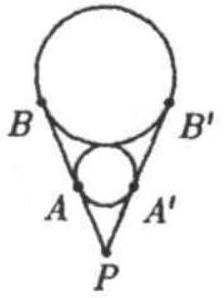
\includegraphics[width=\textwidth]{images/problem_image_1.jpg}

\section*{Solution}
(B)
Connect \(P O, B O, A O_{l}\). Since \(P A=A B, O B \perp P B, O_{1} A \perp P B\), \(P B=P A+A B=8, \quad O B=2 r\).\\
\(P O=2 O O^{\prime}=2(R+r)=2(2 r+r)=6 r\)\\
By the Pythagorean Theorem in right triangle \(P O B\), \(P O^{2}=O B^{2}+P B^{2}\).\\
\(64+4 r^{2}=36 r^{2} \quad \Rightarrow \quad r^{2}=2\)\\
\centering
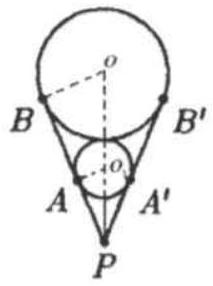
\includegraphics[width=\textwidth]{images/reasoning_image_1.jpg}

The area of the smaller circle is \(2 \pi\).

\end{document}
